\documentclass[10pt]{beamer}
\usetheme[
%%% options passed to the outer theme
%    hidetitle,           % hide the (short) title in the sidebar
%    hideauthor,          % hide the (short) author in the sidebar
%    hideinstitute,       % hide the (short) institute in the bottom of the sidebar
%    shownavsym,          % show the navigation symbols
%    width=2cm,           % width of the sidebar (default is 2 cm)
%    hideothersubsections,% hide all subsections but the subsections in the current section
%    hideallsubsections,  % hide all subsections
    left               % right of left position of sidebar (default is right)
%%% options passed to the color theme
%    lightheaderbg,       % use a light header background
  ]{AAUsidebar}

% If you want to change the colors of the various elements in the theme, edit and uncomment the following lines
% Change the bar and sidebar colors:
%\setbeamercolor{AAUsidebar}{fg=red!20,bg=red}
%\setbeamercolor{sidebar}{bg=red!20}
% Change the color of the structural elements:
%\setbeamercolor{structure}{fg=red}
% Change the frame title text color:
%\setbeamercolor{frametitle}{fg=blue}
% Change the normal text color background:
%\setbeamercolor{normal text}{bg=gray!10}
% ... and you can of course change a lot more - see the beamer user manual.


\usepackage[utf8]{inputenc}
\usepackage[english]{babel}
\usepackage[T1]{fontenc}
% Or whatever. Note that the encoding and the font should match. If T1
% does not look nice, try deleting the line with the fontenc.
\usepackage{helvet}

%Custom packages
\usepackage{graphicx}
\graphicspath{{graphics/}}

% colored hyperlinks
\newcommand{\chref}[2]{%
  \href{#1}{{\usebeamercolor[bg]{AAUsidebar}#2}}%
}

\title[CHINESE WALL]% optional, use only with long paper titles
{THE CHINESE WALL SECURITY POLICY}

\subtitle{Dr. David F.C. Brewer and Dr. Michael J. Nash, 1989}  % could also be a conference name

\date{November 06, 2015}

\author[Mikael Elki\ae r Christensen] % optional, use only with lots of authors
{
  Mikael Elki\ae r Christensen\\
  \href{mailto:michri11@student.aau.dk}{{\tt michri11@student.aau.dk}}
}
% - Give the names in the same order as they appear in the paper.
% - Use the \inst{?} command only if the authors have different
%   affiliation. See the beamer manual for an example

\institute[
%  {\includegraphics[scale=0.2]{aau_segl}}\\ %insert a company, department or university logo
  Department of Computer Science\\
  Aalborg University\\
  Denmark
] % optional - is placed in the bottom of the sidebar on every slide
{% is placed on the title page
  Department of Computer Science\\
  Aalborg University\\
  Denmark
  
  %there must be an empty line above this line - otherwise some unwanted space is added between the university and the country (I do not know why;( )
}


% specify a logo on the titlepage (you can specify additional logos an include them in 
% institute command below
\pgfdeclareimage[height=1.5cm]{titlepagelogo}{AAUgraphics/aau_logo_new} % placed on the title page
%\pgfdeclareimage[height=1.5cm]{titlepagelogo2}{graphics/aau_logo_new} % placed on the title page
\titlegraphic{% is placed on the bottom of the title page
  \pgfuseimage{titlepagelogo}
%  \hspace{1cm}\pgfuseimage{titlepagelogo2}\textsl{}
}


\begin{document}
% the titlepage
{\aauwavesbg%
\begin{frame}[plain,noframenumbering] % the plain option removes the sidebar and header from the title page
  \titlepage
\end{frame}}
%%%%%%%%%%%%%%%%

\section{Introduction}

\begin{frame}{Who is the enemy?}{}
	\begin{columns}
		\begin{column}{.45\textwidth}
			\includegraphics[width=\textwidth]<2->{graphics/computerninja}
		\end{column}
		\begin{column}{.45\textwidth}
			\includegraphics[width=\textwidth]<3>{graphics/gordongekko}
		\end{column}
	\end{columns}
\end{frame}

\subsection{Background}
\begin{frame}{Background}{}
	\begin{itemize}
		\item Coined in 1929 following the Wall Street crash
		\item Chinese Wall policies are already in use
		\begin{itemize}
			\item Not necessarily digital
			\item Can have authority of law
		\end{itemize}
		\item Other terms, as some find the original offensive
		\begin{itemize}
			\item "Screen", "firewall", "cone of silence", and "ethical wall"
		\end{itemize}
	\end{itemize}
\end{frame}

\subsection{Relevance}
\begin{frame}{Relevance}{}
	\begin{itemize}
		\item Before 1989, most security policies were military
		\begin{itemize}
			\item E.g. Bell-LaPadula (more about this later)
		\end{itemize}
		\item Need of something that holds up in court
		\item Relevant anywhere conflicts of interest can exist
	\end{itemize}
\end{frame}

%%%%%%%%%%%%%%%%

\section{Bell-LaPadula}

\begin{frame}{Bell-LaPadula}{}
	\begin{itemize}
		\item Proposed by Bell and LaPadula in 1973
		\item Security policy model
		\item Designed for military use
	\end{itemize}
\end{frame}

\subsection{Terminology}
\begin{frame}
	\frametitle{Terminology}
	
	\begin{itemize}
		\item \textbf{Security Label}
		\item \textbf{Object} -- Data or program
			\begin{itemize}
				\item \textbf{Classification} -- Minimum security level
				\item \textbf{Category} -- Security group(s)
			\end{itemize}
		\item \textbf{Subject} -- Person or program
			\begin{itemize}
				\item \textbf{Clearance} -- Maximum security level
				\item \textbf{Need-to-know} -- Security group(s)
			\end{itemize}
	\end{itemize}
\end{frame}

\subsection{Access rules}
\begin{frame}
	\frametitle{Access rules}
	
	\begin{description}
		\item[Simple security:] access is granted only if the subject's clearance is \textit{greater} than the object's classification and the subject's need-to-know \textit{includes} the object's category(ies)
		\item[*-property:] write access is granted only if the output object's classification is \textit{greater} than the classification of all input objects, and its category \textit{includes} the category(ies) of all input objects.
	\end{description}
\end{frame}

\subsection{Example}
\begin{frame}
	\frametitle{Example}
	
	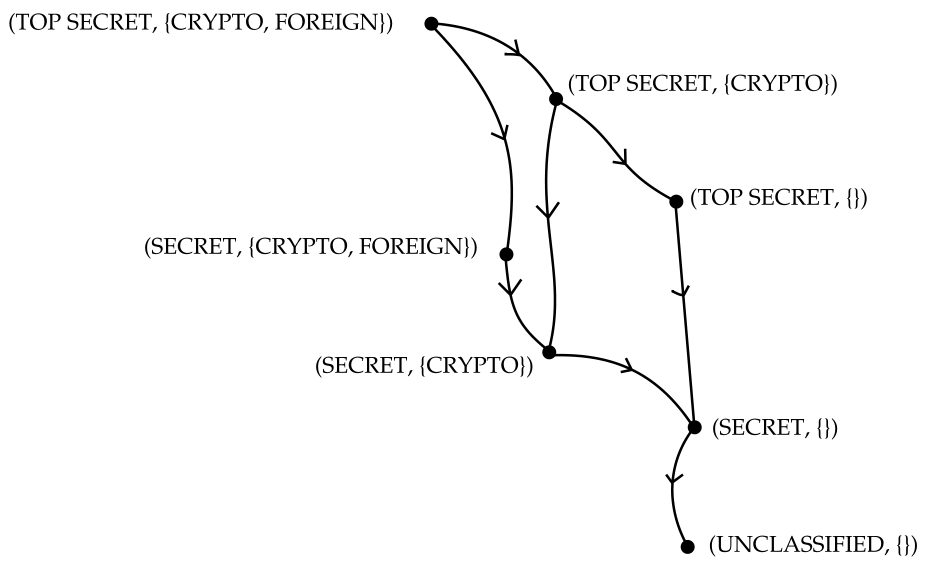
\includegraphics[width=\textwidth]{graphics/blp_lattice}
\end{frame}

\begin{frame}
	\frametitle{Example (2)}
	
	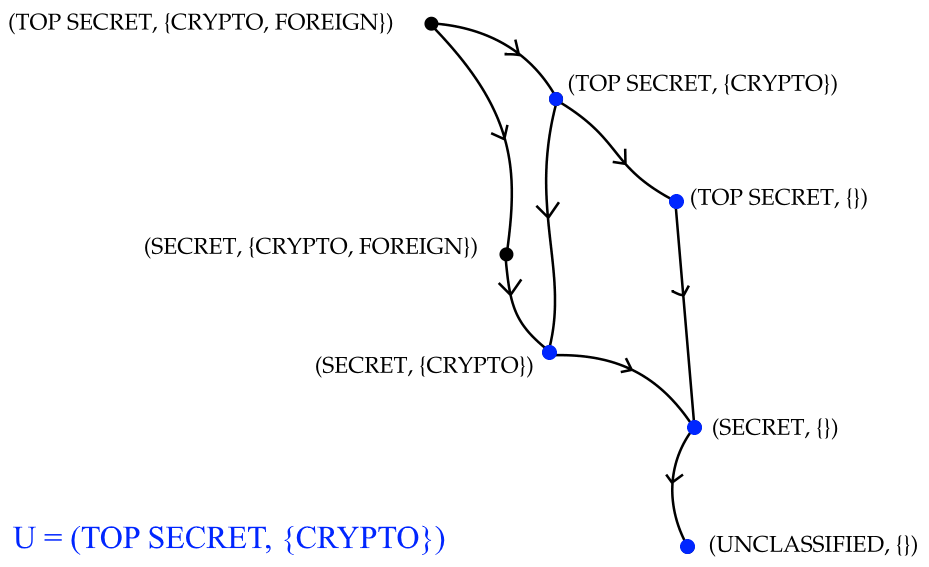
\includegraphics[width=\textwidth]{graphics/blp_lattice_2}
\end{frame}

%%%%%%%%%%%%%%%

\section{Chinese Wall}

\begin{frame}
	\frametitle{Fundamentals}
	
	\begin{itemize}
		\item Terminology
		\begin{itemize}
			\item Object
			\item Subject
			\item Company Dataset (CD)
			\item Conflict of Interest Class (COIC)
		\end{itemize}
		\item Main difference: At most one CD in each COIC, starting with free choice
	\end{itemize}
\end{frame}

\subsection{Abstract Example}
\begin{frame}
	\frametitle{Abstract Example}
	
	See blackboard...
\end{frame}

\subsection{Hierarchical Example}
\begin{frame}
	\frametitle{Hierarchical Example}
	
	Users $X, Y$
	\begin{tikzpicture}[scale=0.7]
	\node (v3) at (-2,0) {};
	\node (v2) at (-3,0) {};
	\node (v1) at (-3,-1) {};
	\node (v6) at (-2,-1) {};
	\node (v4) at (-1,0) {};
	\node (v5) at (-1,-1) {};
	\draw (v1) -- (v2) -- (v3) -- (v4) -- (v5);
	\node (v7) at (-2,1) {A};
	\draw (v6) -- (v3) -- (v7);
	
	\node (v14) at (0,1) {};
	\node (v13) at (2,1) {B};
	\node (v10) at (2,0) {};
	\node (v9) at (1,0) {};
	\node (v8) at (1,-1) {};
	
	\node (v12) at (3,-1) {};
	\node (v11) at (3,0) {};
	\draw (v8) -- (v9) -- (v10) -- (v11) -- (v12);
	\draw (2,-1) -- (v10) -- (v13) -- (v14) -- (v7);
	\node (v15) at (0,2) {C};
	\draw  (v14) edge (v15);
		
	\node (v30) at (4,2) {};
	\node (v40)at (8,2) {D};
	\node (v23) at (8,1) {};
	\node (v22) at (6,1) {K};
	\node (v24) at (10,1) {J};
	\node (v25) at (10,0) {};
	\node (v28) at (9,0) {};
	\node (v27) at (9,-1) {};
	\node (v26) at (10,-1) {};
	\node at (11,-1) {};
	\node (v29) at (11,0) {};
	\node (v18) at (6,0) {};
	\node (v17) at (5,0) {};
	\node (v16) at (5,-1) {};
	\node (v21) at (6,-1) {};
	\node (v20) at (7,-1) {};
	\node (v19) at (7,0) {};
	\draw (v16) -- (v17) -- (v18) -- (v19) -- (v20);
	\draw (v21) -- (v18) -- (v22) -- (v23) -- (v24) -- (v25) -- (v26);
	\draw (v27) -- (v28) -- (v25) -- (v29) -- (11,-1);
	\draw (v23) -- (v40) -- (v30) -- (v15);
	\node (v31) at (4,3) {O};
	\draw  (v30) edge (v31);
	\end{tikzpicture}
\end{frame}

\subsection{Access rules}
\begin{frame}
	\frametitle{Access rules}
	
	\begin{columns}
		\begin{column}{.45\textwidth}
			\begin{block}{Simple security}
				Access is only granted if the object requested
				\begin{enumerate}
					\item is in the \textit{same company dataset} as an object already accessed by that subject, i.e. within the Wall, \textit{or}
					\item belongs to an \textit{entirely different conflict of interest class}.
				\end{enumerate}
			\end{block}
		\end{column}
		\begin{column}{.45\textwidth}
			\begin{block}{*-property}
				Write access is only permitted if
				\begin{enumerate}
					\item access is permitted by the simple security rule, and
					\item no object can be read which is in a different company dataset to the one for which write access is requested and contains unsanitized information.
				\end{enumerate}
			\end{block}
		\end{column}
	\end{columns}
\end{frame}

\subsection{Sanitization}
\begin{frame}
	\frametitle{Sanitization}
	
	\begin{itemize}
		\item Not all data within a company is sensitive
		\item It can be necessary to share data between users
		\item Assumed possible by de-privatizing
		\item Simply solved by adding extra CD within its own COIC
	\end{itemize}
\end{frame}

{\aauwavesbg
\begin{frame}[plain,noframenumbering]
	\finalpage{Questions?}
\end{frame}}
%%%%%%%%%%%%%%%%

\end{document}
